\section{Theorie}
\label{sec:Theorie}

\subsection{Motivation und Zielsetzung}

Ziel dieses Versuches ist es, die Erzeugung eines Vakuums mithilfe von zwei
verschiedenen Pumpentypen zu verstehen und durchzuführen.
Durch Aufnahme einer Evakuierungskurve sowie einer Leckratenmessung können die
Hestellerangaben bezüglich des Saugvermögens der Pumpen überprüft werden.
Aufgrund des immer geringeren Atmosphärendrucks in großen Höhen ist die Vakuumphysik
in technischen Anwendungen von großer Bedeutung, um beispielweise Werkstoffe für
die Luft- und Raumfahrt zu entwickeln und zu testen.
Auch auf dem Boden müssen viele Prozesse im Vakuum stattfinden, um den störenden
Einfluss der Atmosphäre zu eliminieren. Ein Beispiel hierfür sind Teilchenbeschleuniger,
die ein sehr gutes Vakuum erforden, um Wechselwirkungen mit Gasteilchen zu verhindern.

\subsection{Theoretische Grundlagen}

Da ein perfektes Vakuum in der Praxis unmöglich zu erreichen ist, wird das Vakuum über verschiedene
Druckbereiche definiert. Erst ab Drücken von $p < \qty{300}{\milli\bar}$ wird der Begriff Vakuum verwendet,
da größere Drücke noch auf der Erdoberfläche anzutreffen sind.
In \autoref{tab:druecke} sind die verschiedenen Druckbereiche mit der dazugehörigen Definition des Vakuums
aufgeführt. In diesem Versuch wird maximal die Größenordnung eines Hochvakuums erreicht.
\begin{table}[H]
    \centering
    \caption{Druckbereiche in der Vakuumtechnik \cite{Pfeiffer_Vakuum}.}
    \label{tab:druecke}
    \begin{tabular}{c|c}
        \toprule
        Druckbereich & Druck / $\unit{\milli\bar}$\\
        \midrule
        Grobvakuum & $300 - 1$\\
        Feinvakuum & $1 - 10^{-3}$\\
        Hochvakuum & $10^{-3} - 10^{-8}$\\
        Ultrahochvakuum & $<10^{-8}$\\
        \bottomrule
    \end{tabular}
\end{table}
Die simpelste Beschreibung eines Gases liefert das Modell des idealen Gases. Hier werden alle Gasatome als punktförmig angenommen und
die Teilchen wechselwirken nicht untereinander. Es finden lediglich elastische Stößen untereinander und mit den Außenwänden statt.
Es gilt dann die Zustandsgleichung
\begin{equation}
    \label{eqn:gasgleichung}
    p V=N k_{\text{B}} T
\end{equation}
wobei $p$ für den Druck, $V$ für das Volumen, $N$ für die Teilchenzahl und $T$ für die Temperatur steht, $k_{\text{B}}$ ist die Boltzmann Konstante.
Bei konstanter Temperatur folgt sofort das Boyle-Mariott’schen Gesetz
\begin{equation}
    \label{eqn:bmgesetz}
    p V=const
\end{equation}
was einen antiproportionalen Zusammenhang zwischen $p$ und $V$ vorhersagt.
Die getroffenen Anahmen sind jedoch nicht für alle Komponenten der Atmosphäre anwendbar, zum Beispiel die stark polarisierten
Wassermoleküle im Wasserdampf wechselwirken stark miteinander, und die oben beschriebenen Zusammenhänge verlieren ihre Gültigkeit.
Um niedrige Drücke erreichen zu können, müssen derartige Verunreinigungen aus dem System entfernt werden.\\

Die gemeinsame Bewegung der Gasteilchen wird auch als \textit{Strömung} bezeichnet und hängt stark vom vorherrschenden Druck ab.
Je geringer der Druck, desto weniger Gasteilchen befinden sich im System und umso weniger Stöße finden untereinander statt.
Der durchschnittliche Weg, den ein Teilchen ohne Wechselwirkungen zurücklegen kann, wird als \textit{mittlere freie Weglänge} bezeichnet
und nimmt mit sinkendem Druck stark zu.
Ein Maß für die vorliegende Strömung ist die Knudsenzahl
\begin{equation}
    \notag
    K_{\text{n}} = \frac{\bar{l}}{d}
\end{equation}
bei der $\bar{l}$ für die mittlere freie Weglänge und $d$ für den Durchmesser des Rohres steht.
In \autoref{fig:stroemungen} sind die verschiedenen Arten von Strömungen in Abhängigkeit der Knudsenzahl
dargestellt.
\begin{figure}[H]
    \centering
    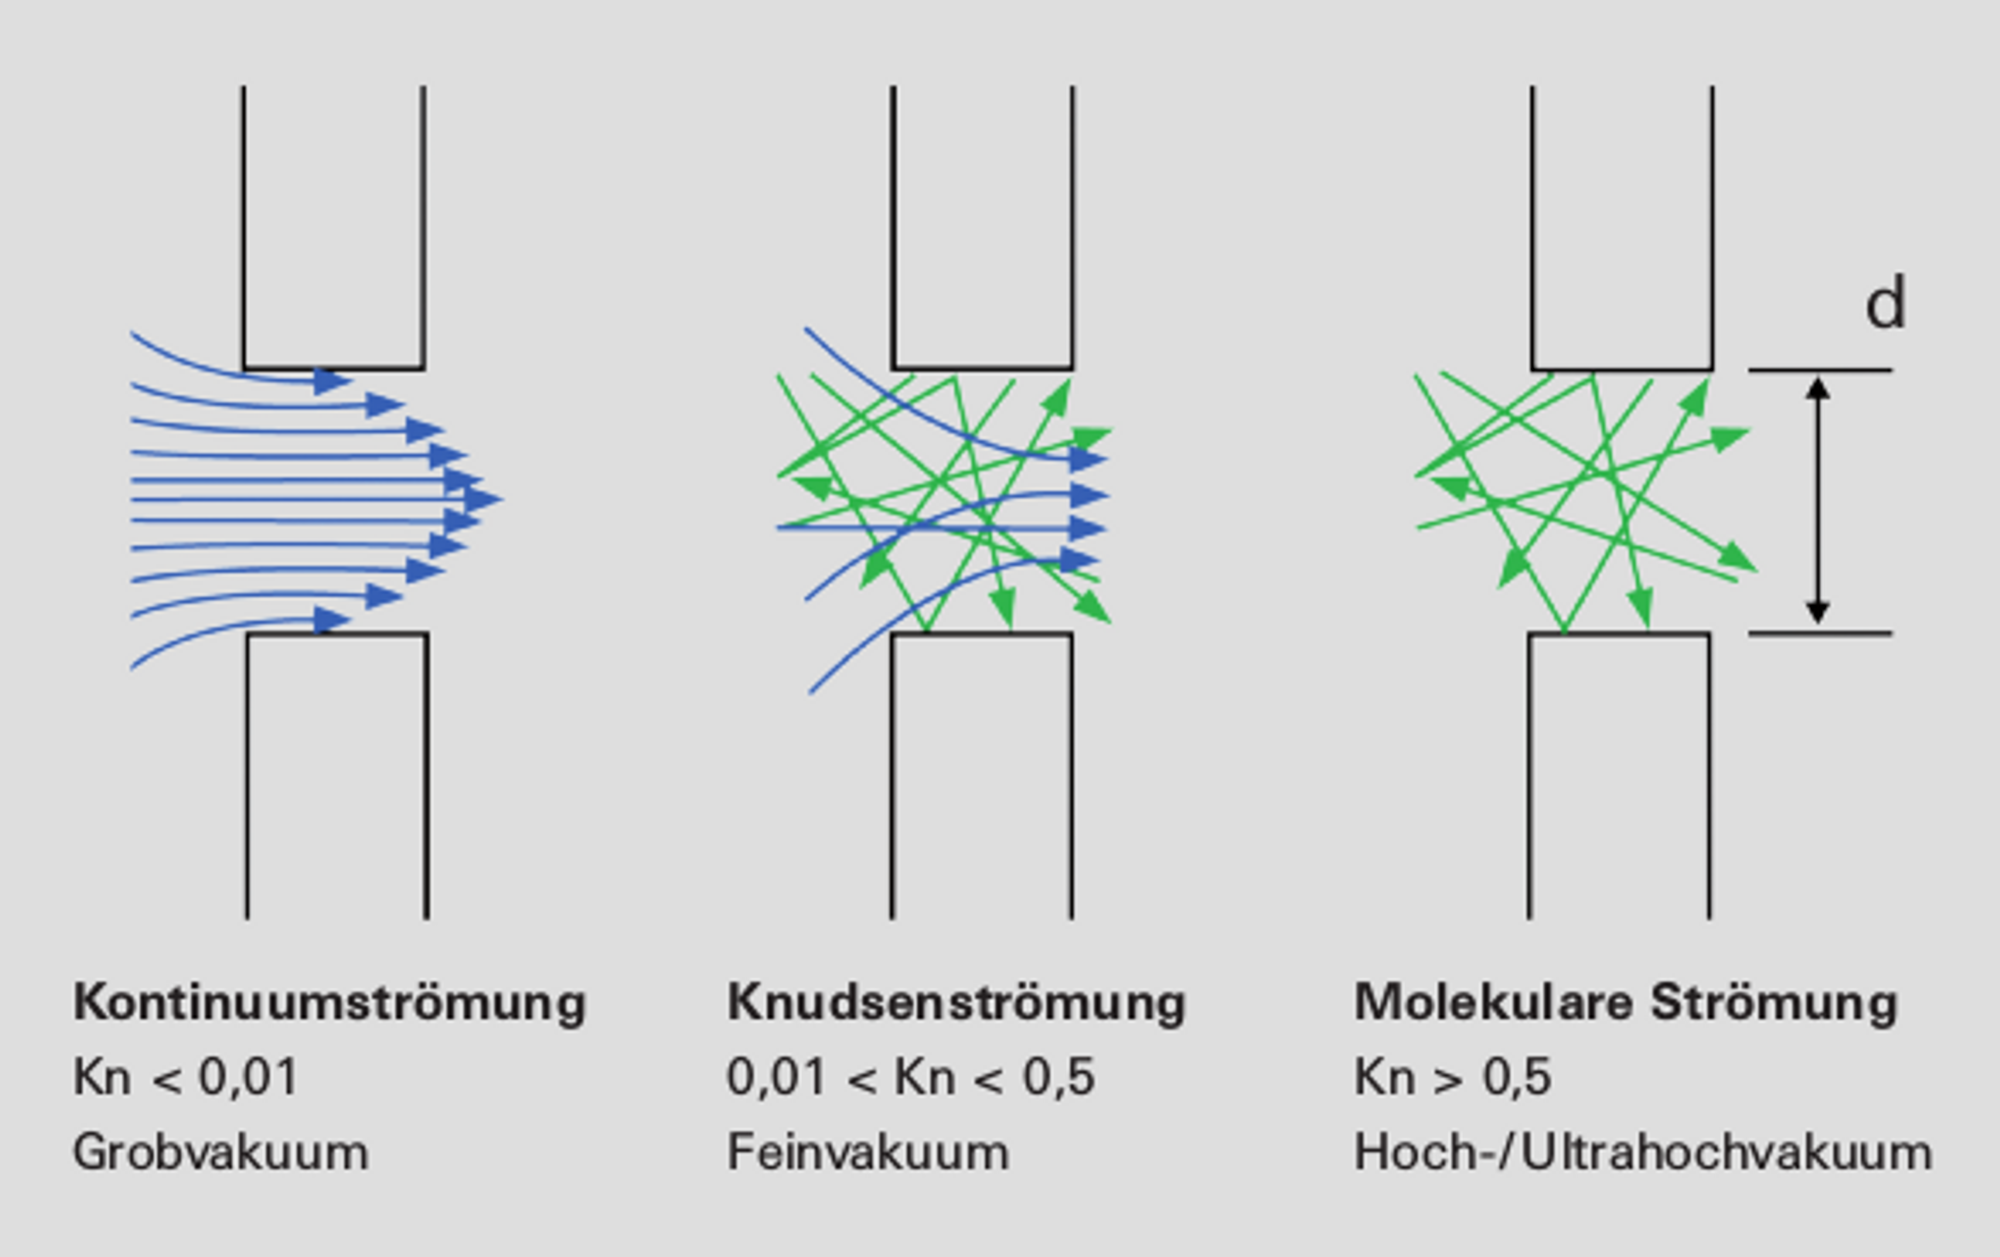
\includegraphics[width=0.6\textwidth]{content/pics/stroemung.png}
    \caption{Übersicht über die verschiedenen Strömungsarten \cite{Pfeiffer_Vakuum}.}
    \label{fig:stroemungen}
\end{figure}
Im Grobvakuum liegt laminare Strömung vor, die Gasteilchen bewegen sich also in zueinander parallelen Schichten.
Nimmt der Druck ab, so werden Wechselwirkungen zwischen den Teilchen immer seltener, bis schließlich nur noch
Stöße mit den Wänden stattfinden. Alle Teilchen bewegen sich unabhängig von einander und man nennt dies molekulare
Strömung.

\subsection{Vakuumerzeugung}

Um ein Vakuum zu erzeugen wird eine Pumpe benötigt, die das Gas gegen den Atmosphärendruck aus dem System pumpt.
Das Saugvermögen einer Pumpe ist über die Änderung des Volumens definiert:
\begin{equation}
    \label{eqn:saugvermoegen}
    S = \frac{\text{d}V}{\text{d}t}.
\end{equation}
Als Saugleistung bezeichnet man das Produkt aus Saugvermögen und Druck
\begin{equation}
    \label{eqn:saugleistung}
    q_{\text{pV}} = S \cdot P.
\end{equation}
In der Praxis wird die theoretische Saugleistung $S_0$ einer Pumpe nie ganz erreicht, da das sich zwangsläufig davorbefindende
Rohr einen Leitwert $L$ hat, der die Gasmenge begrenzt. Dieser kann analog zu einem reziproken elektrischen Widerstand verstanden werden.
Daher wird die effektive Saugleistung $S_{\text{eff}}$ verwendet, die sich gemäß
\begin{equation}
    \label{eqn:saugleistung_eff}
    \frac{1}{S_{\text{eff}}} = \frac{1}{S_{0}} + \frac{1}{L}
\end{equation}
berechnet. In der Regel ist das Saugvermögen einer Pumpe nicht konstant, sondern Abhängig vom Druck.
Nimmt man jedoch vereinfacht ein konstantes Saugvermögen an, so kann durch zeitliches Ableiten der Zustandsgleichung \eqref{eqn:gasgleichung}
die Differentialgleichung
\begin{equation}
    \notag
    \dot{p} \cdot V = -p \cdot S
\end{equation}
aufgestellt werden. Deren Lösung beschreibt die sogenannte Evakuierungskurve $p(t)$, die den zeitlichen Verlauf des Druckes gemäß
\begin{equation}
    \label{eqn:evakuierungskurve}
    p(t) = p_0 \cdot \exp{\left(-\frac{S}{V}\,t\right)}.
\end{equation}
beschreibt.
Ein System ist nie vollständig dicht, der Druckabfall durch verschiedene Lecks wird du die Leckrate
\begin{equation}
    \label{eqn:leckrate}
    Q = \frac{\symup{\Delta} p}{\symup{\Delta} t}\cdot V
\end{equation}
beschrieben, dabei steht $\symup{\Delta} p$ für den Druck, der in der Zeit $\symup{\Delta} t$ dazugekommen ist.
Über die Leckrate $Q$ lässt sich ebenfalls das zuvor beschriebene Saugvermögen $S$ berechnen mit der Formel
\begin{equation}
    \label{eqn:s_leck}
    S = \frac{Q}{p_{\text{G}}}.
\end{equation}
Dafür muss der Gleichgewichtsdruck $p_{\text{G}}$ bekannt sein. Bei diesem Druck gleicht sich die Saugleistung der Pumpe genau mit den
Undichtigkeiten der Lecks aus, sodass ein Gleichgewicht entsteht. \\
Für unterschiedliche Druckbereiche gibt es verschiedene Funktionsprinzipien von Pumpen, in diesem Versuch werden zwei Typen von Vakuumpumpen verwendet:
\begin{enumerate}
    \item Die \textbf{Drehschieberpumpe} zählt zur Kategorie der Transport- bzw. Verdrängerpumpen, das Arbeitsprinzip ist also der Abtransport von Gas
    durch Ansaugung und anschließende Verdrängung. Eine Skizze ihres Aufbaus ist in \autoref{fig:Drehschieberpumpe} zu sehen.
    \begin{figure}[H]
        \centering
        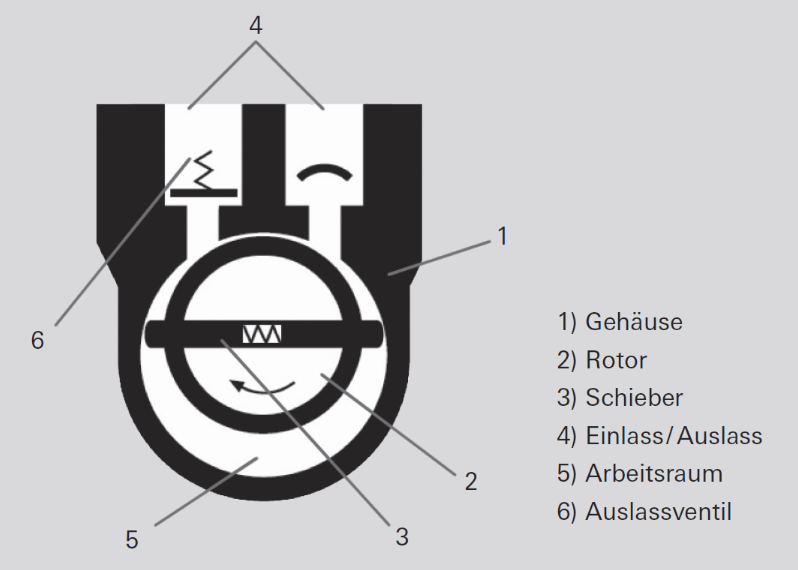
\includegraphics[width=0.6\textwidth]{content/pics/drehschieberpumpe.png}
        \caption{Schematische Darstellung des Aufbaus einer Drehschieberpumpe \cite{Pfeiffer_Drehschieberpumpe}.}
        \label{fig:Drehschieberpumpe}
    \end{figure}
    Im Gehäuse befindet ein sich drehender Rotor, der Schieber besitzt, um den Arbeitsraum zu teilen und abzudichten.
    Zu Beginn eines Arbeitstaktes strömt Gas durch den Einlass in den Arbeitsraum, da dieser sich expandiert und somit ein Druckgefälle vorliegt.
    Dannach wird der Raum durch den zweiten Schieber verschlossen und das Gas komprimiert. Sobald der Druck den Atmosphärendruck übersteigt,
    öffnet das Auslassventil und das Gas entweicht aus der Pumpe. In der Pumpe befindet sich zu jeder Zeit eine kleine Menge Öl, das
    eine Schmierung der Lager sowie eine saubere Abdichtung der Schieber und Ventile gewährleistet. Aufgrund der limitierten Kompressionsfähigkeit
    im Arbeitsraum durch konstruktionstechnisch bedingte Restvolumina ist der Druckbereich der Pumpe limitiert.
    Einstufige Ausführungen erreichen typischerweise Enddrücke von $\qty{0.1}{\milli\bar}$, durch weitere Stufen kann dies weiter verringert werden.
    Eine Drehschieberpumpe eignet sich somit zur Erzeugung eines Vorvakuus, das anschließend mit Pumpen anderer Bauart verfeinert werden kann.
    \item Bei gegebenen Vorvakuum kann der Druck mithilfe einer \textbf{Turbomolekularpumpe} weiter verringert werden.
    In \autoref{fig:Turbo} ist der grobe Aufbau dargestellt.
    Die Turbomolekularpumpe zählt zu den kinetischen Pumpen. Ein Rotor mit Schaufeln führt den Gasteilchen kinetische Energie zu, sodass sie
    sich zwischen Rotor und Stator entlang aus dem System heraus bewegen. Das Funktionsprinzip kann somit mit dem einer Turbine verglichen werden. Der
    Stator muss mit hoher Drehzahl betrieben werden, damit der Energieübertrag relevant gegenüber der thermischen Energie der Teilchen ist.
    Das Vorvakuum wird benötigt, um die zufälligen Kollisionen der Gasteilchen untereinander zu unterdrücken, da diese dem Pumpprozess entgegenwirken
    würden. Im Gegenzug können Drücke im Bereich $\qty{1e-3}{\milli\bar}$ und $\qty{1e-10}{\milli\bar}$ erreicht werden \cite{Pfeiffer_Turbomolekularpumpen},
    was bereits einem Hochvakuum entspricht.
    \begin{figure}[H]
        \centering
        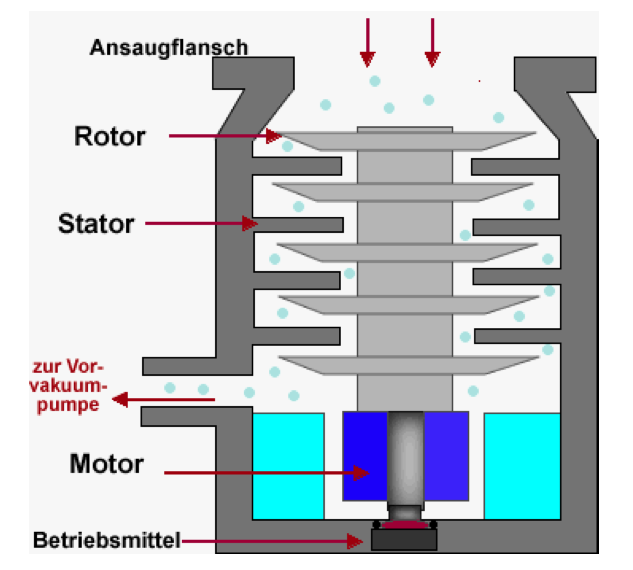
\includegraphics[width=0.6\textwidth]{content/pics/turbo.png}
        \caption{Schematische Darstellung des Aufbaus einer Drehschieberpumpe \cite{Turbopumpe}.}
        \label{fig:Turbo}
    \end{figure}
\end{enumerate}

\subsection{Vakuummessung}
Um die Güte des erzeugten Vakuums zu messen, gibt es je nach Druckbereich verschiedene Messmethoden bzw. Messgeräte.
\begin{itemize}
    \item Eine \textbf{Pirani-Messröhre} nutzt die Druckabhängigkeit der Wärmeleitfähigkeit von Gasen aus. Durch einen Draht wird
    soviel Strom geleitet, sodass dieser anfängt zu glühen. Je geringer der Druck, desto schlechter wird die Wärme abgeführt und der
    Draht wird heißer. Dadurch erhöht sich der Widerstand, was mithilfe einer Messbrücke nachgewiesen werden kann. Der Widerstand ist somit
    proportional zum Druck, solange dieser nicht kleiner als $\qty{1e-4}{\milli\bar}$ wird, dann überwiegt die Wärmestrahlung.
    Auch bei Drücken größer $\qty{10}{\milli\bar}$ ist die Wärmeleitfähigkeit unabhängig vom Druck, dies begrenzt das Messfenster nach oben. \cite{Druckmessung}
    \item Das \textbf{Piezo-Membranvakuummeter} nutzt die den Druck ausgelöste Kraft auf eine Fäche. Auf einer Membran platzierte Piezo-Kristalle
    verändern wegen deren Durchbiegung ihre Länge und somit den Widerstand, der dann gemessen werden kann. Diese Messmethode bietet eine hohe Präzision,
    ab Drücken unter $\qty{1e-5}{\milli\bar}$ wird die Kraft und somit die Durchbiegung jedoch zu gering. \cite{Druckmessung}
    \item Niedrigere Druckbereiche können mit \textbf{Ionisationsvakuumetern} gemessen werden, diese Beruhen auf der Ionisation der Gasatome mithilfe von
    Elektronen. Zwischen einer Anode und Kathode werden Elektronen beschleunigt, die Hüllenelektronen der Gasatome aus der äußeren Schale stoßen.
    Die Gasatome sind anschließend Ionisiert und verursachen einen messbaren Ionisationsstrom. Da mit sinkendem Druck die Anzahl an Gasatomen abnimmt,
    ist dieser Strom proportional zum Druck. Es wird zwischen \textit{Kaltkathoden-} und \textit{Heißkathodenvakuumetern} unterschieden.
    Beim \textit{Kaltkathodenvakuumeter} werden die Elektronen durch Feldemmision erzeugt, während das \textit{Heißkathodenvakuumeter} den
    glühelektrischen Effekt verwendet. Um den Messbereich zu erweitern werden die Elektronen durch ein Magnetfeld geschickt, die resultierenden
    Kreisbahnen erhöhen die Stoßwahrscheinlichkeit mit den Atomen signifikant. Somit lassen sich auf diese Art Drücke von bis zu $\qty{1e-10}{\milli\bar}$
    nachweisen. \cite{Druckmessung}
\end{itemize}